\documentclass[runningheads,a4paper]{llncs}
\usepackage{color}
\usepackage{amssymb}
\usepackage{amsmath}
\usepackage{tikz}
\usepackage{pgfplots}
\usetikzlibrary{positioning}
\usetikzlibrary{calc}
\usetikzlibrary{arrows.meta, automata, positioning, calc}
\usepackage{xcolor}
\usepackage{pgf}
\usepackage{tikz}
\usetikzlibrary{arrows,automata,calc}

\begin{document}

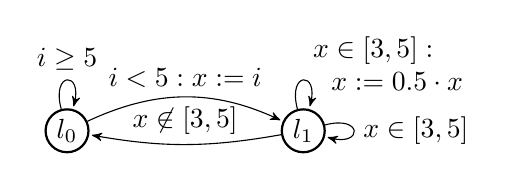
\begin{tikzpicture}[->,>=stealth',shorten >=1pt,auto,node distance=3cm]
\tikzstyle{every state}=[fill=none,draw=black,text=black,inner sep=1.5pt, minimum size=11pt,thick]
  \node[state] (l0) at (0,0) {$l_0$};
  \node[state] (l1) at (3,0) {$l_1$};
  \path
    (l0) edge[loop above] node[above, align=left] 
        {$i \geq 5$}
    (l0) edge[bend left=25] node[above, align=center] 
        {$i < 5: x := i$} 
    (l1)
    (l1) edge[bend left=10] node[above, align=left] 
        {$x \not\in [3, 5]$} 
    (l0)
    (l1) edge[loop right] node[right, align=left] {%
         $x \in [3, 5]$}
    (l1) edge[loop above] node[right, align=left] {%
        $x \in [3, 5] :$\\ $~~x := 0.5 \cdot x$\\%
    }
    (l1) 
  ;
\end{tikzpicture}

\end{document}